Um mapa � a representa��o reduzida e simplificada de uma localidade. Essa redu��o, que � feita com o uso de uma escala, mant�m a propor��o do espa�o representado em rela��o ao espa�o real. 
Certo mapa tem escala 1 : 58 000 000.

\begin{figure}[h]
\centering
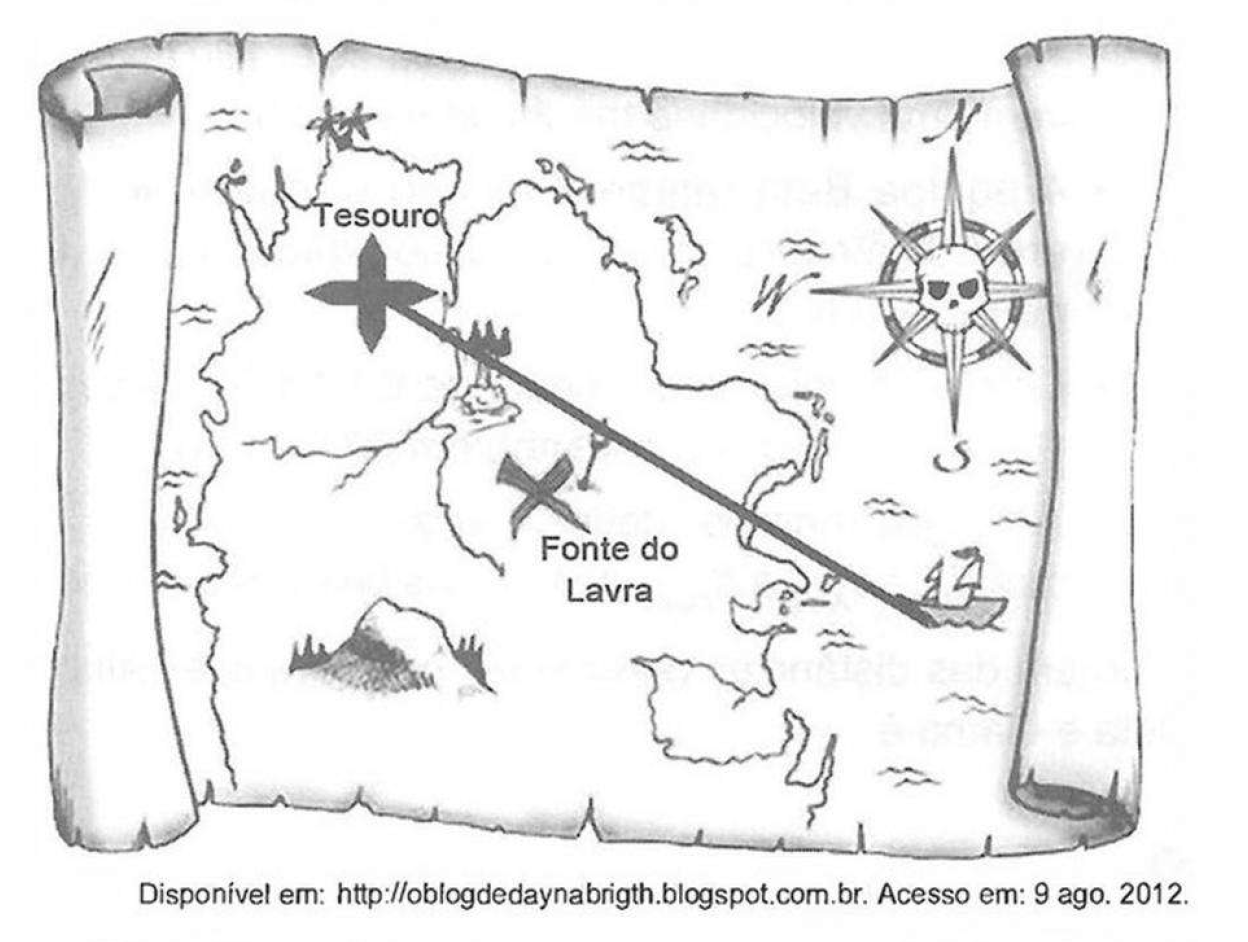
\includegraphics[width=8cm]{../figuras/q167-2018}
\end{figure}

Considere que, nesse mapa, o segmento de reta que liga o navio � marca do tesouro me�a 7,6 cm. 
A medida real, em quil�metro, desse segmento de reta � 
\begin{enumerate}
\item[a)]4408
\item[b)]7632
\item[c)]44080
\item[d)]76316
\item[e)]440800
\end{enumerate}